

\tikzset{every picture/.style={line width=0.75pt}} %set default line width to 0.75pt        

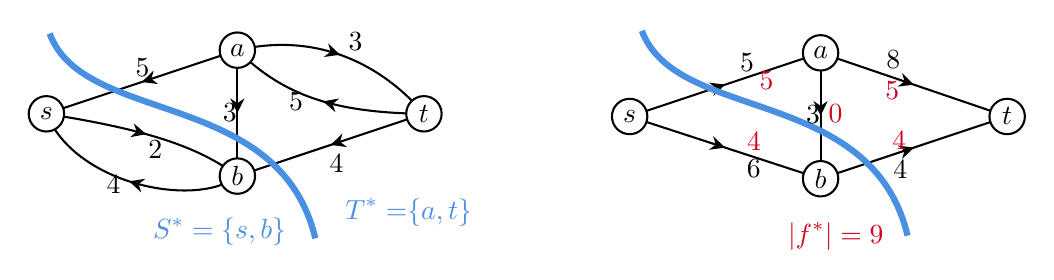
\begin{tikzpicture}[x=0.5pt,y=0.5pt,yscale=-1,xscale=1]
%uncomment if require: \path (0,176); %set diagram left start at 0, and has height of 176

%Straight Lines [id:da09123496908131157] 
\draw    (296,70) -- (161.17,115) ;
\draw [shift={(228.59,92.5)}, rotate = 341.54] [fill={rgb, 255:red, 0; green, 0; blue, 0 }  ][line width=0.08]  [draw opacity=0] (10.72,-5.15) -- (0,0) -- (10.72,5.15) -- (7.12,0) -- cycle    ;
%Straight Lines [id:da19597903283531382] 
\draw [color={rgb, 255:red, 0; green, 0; blue, 0 }  ,draw opacity=1 ]   (161.17,24) -- (23.17,70) ;
\draw [shift={(92.17,47)}, rotate = 341.57] [fill={rgb, 255:red, 0; green, 0; blue, 0 }  ,fill opacity=1 ][line width=0.08]  [draw opacity=0] (10.72,-5.15) -- (0,0) -- (10.72,5.15) -- (7.12,0) -- cycle    ;
%Curve Lines [id:da003967634620389404] 
\draw [color={rgb, 255:red, 0; green, 0; blue, 0 }  ,draw opacity=1 ]   (161.17,24) .. controls (224.88,9.25) and (270.88,40.25) .. (296,70) ;
\draw [shift={(235.42,27.34)}, rotate = 198.02] [fill={rgb, 255:red, 0; green, 0; blue, 0 }  ,fill opacity=1 ][line width=0.08]  [draw opacity=0] (10.72,-5.15) -- (0,0) -- (10.72,5.15) -- (7.12,0) -- cycle    ;
%Curve Lines [id:da9544255371930271] 
\draw    (296,70) .. controls (231.88,69.25) and (194.88,57.25) .. (161.17,24) ;
\draw [shift={(223.07,61.05)}, rotate = 15.31] [fill={rgb, 255:red, 0; green, 0; blue, 0 }  ][line width=0.08]  [draw opacity=0] (10.72,-5.15) -- (0,0) -- (10.72,5.15) -- (7.12,0) -- cycle    ;
%Curve Lines [id:da14332777144371744] 
\draw [color={rgb, 255:red, 0; green, 0; blue, 0 }  ,draw opacity=1 ]   (23.17,70) .. controls (88.88,80.25) and (131.88,92.25) .. (161.17,115) ;
\draw [shift={(95.33,84.71)}, rotate = 195.08] [fill={rgb, 255:red, 0; green, 0; blue, 0 }  ,fill opacity=1 ][line width=0.08]  [draw opacity=0] (10.72,-5.15) -- (0,0) -- (10.72,5.15) -- (7.12,0) -- cycle    ;
%Curve Lines [id:da2638365923485928] 
\draw    (161.17,115) .. controls (132.88,138.25) and (44.88,122.25) .. (23.17,70) ;
\draw [shift={(82.94,118.8)}, rotate = 16.76] [fill={rgb, 255:red, 0; green, 0; blue, 0 }  ][line width=0.08]  [draw opacity=0] (10.72,-5.15) -- (0,0) -- (10.72,5.15) -- (7.12,0) -- cycle    ;
%Straight Lines [id:da47468815088752225] 
\draw [color={rgb, 255:red, 0; green, 0; blue, 0 }  ,draw opacity=1 ]   (161.17,24) -- (161.17,115) ;
\draw [shift={(161.17,69.5)}, rotate = 270] [fill={rgb, 255:red, 0; green, 0; blue, 0 }  ,fill opacity=1 ][line width=0.08]  [draw opacity=0] (10.72,-5.15) -- (0,0) -- (10.72,5.15) -- (7.12,0) -- cycle    ;
%Shape: Ellipse [id:dp954041169370231] 
\draw  [fill={rgb, 255:red, 255; green, 255; blue, 255 }  ,fill opacity=1 ] (10.38,70) .. controls (10.38,62.94) and (16.11,57.21) .. (23.17,57.21) .. controls (30.23,57.21) and (35.96,62.94) .. (35.96,70) .. controls (35.96,77.06) and (30.23,82.79) .. (23.17,82.79) .. controls (16.11,82.79) and (10.38,77.06) .. (10.38,70) -- cycle ;
%Shape: Ellipse [id:dp9013075185816432] 
\draw  [fill={rgb, 255:red, 255; green, 255; blue, 255 }  ,fill opacity=1 ] (283.21,70) .. controls (283.21,62.94) and (288.94,57.21) .. (296,57.21) .. controls (303.06,57.21) and (308.79,62.94) .. (308.79,70) .. controls (308.79,77.06) and (303.06,82.79) .. (296,82.79) .. controls (288.94,82.79) and (283.21,77.06) .. (283.21,70) -- cycle ;
%Shape: Ellipse [id:dp8082050050742036] 
\draw  [fill={rgb, 255:red, 255; green, 255; blue, 255 }  ,fill opacity=1 ] (148.38,24) .. controls (148.38,16.94) and (154.11,11.21) .. (161.17,11.21) .. controls (168.23,11.21) and (173.96,16.94) .. (173.96,24) .. controls (173.96,31.06) and (168.23,36.79) .. (161.17,36.79) .. controls (154.11,36.79) and (148.38,31.06) .. (148.38,24) -- cycle ;
%Shape: Ellipse [id:dp31893054203886095] 
\draw  [fill={rgb, 255:red, 255; green, 255; blue, 255 }  ,fill opacity=1 ] (148.38,115) .. controls (148.38,107.94) and (154.11,102.21) .. (161.17,102.21) .. controls (168.23,102.21) and (173.96,107.94) .. (173.96,115) .. controls (173.96,122.06) and (168.23,127.79) .. (161.17,127.79) .. controls (154.11,127.79) and (148.38,122.06) .. (148.38,115) -- cycle ;

%Straight Lines [id:da18092572046534006] 
\draw    (444.67,71.93) -- (582.67,116.93) ;
\draw [shift={(513.67,94.43)}, rotate = 198.06] [fill={rgb, 255:red, 0; green, 0; blue, 0 }  ][line width=0.08]  [draw opacity=0] (10.72,-5.15) -- (0,0) -- (10.72,5.15) -- (7.12,0) -- cycle    ;
%Straight Lines [id:da026108681541828216] 
\draw    (444.67,71.93) -- (582.67,25.93) ;
\draw [shift={(513.67,48.93)}, rotate = 161.57] [fill={rgb, 255:red, 0; green, 0; blue, 0 }  ][line width=0.08]  [draw opacity=0] (10.72,-5.15) -- (0,0) -- (10.72,5.15) -- (7.12,0) -- cycle    ;
%Straight Lines [id:da4824803197457034] 
\draw    (582.67,25.93) -- (582.67,116.93) ;
\draw [shift={(582.67,71.43)}, rotate = 270] [fill={rgb, 255:red, 0; green, 0; blue, 0 }  ][line width=0.08]  [draw opacity=0] (10.72,-5.15) -- (0,0) -- (10.72,5.15) -- (7.12,0) -- cycle    ;
%Straight Lines [id:da5740743987306038] 
\draw    (582.67,25.93) -- (717.5,71.93) ;
\draw [shift={(650.09,48.93)}, rotate = 198.84] [fill={rgb, 255:red, 0; green, 0; blue, 0 }  ][line width=0.08]  [draw opacity=0] (10.72,-5.15) -- (0,0) -- (10.72,5.15) -- (7.12,0) -- cycle    ;
%Straight Lines [id:da8273834872954168] 
\draw    (582.67,116.93) -- (717.5,71.93) ;
\draw [shift={(650.09,94.43)}, rotate = 161.54] [fill={rgb, 255:red, 0; green, 0; blue, 0 }  ][line width=0.08]  [draw opacity=0] (10.72,-5.15) -- (0,0) -- (10.72,5.15) -- (7.12,0) -- cycle    ;
%Shape: Ellipse [id:dp16280961740768174] 
\draw  [fill={rgb, 255:red, 255; green, 255; blue, 255 }  ,fill opacity=1 ] (431.88,71.93) .. controls (431.88,64.86) and (437.61,59.14) .. (444.67,59.14) .. controls (451.73,59.14) and (457.46,64.86) .. (457.46,71.93) .. controls (457.46,78.99) and (451.73,84.72) .. (444.67,84.72) .. controls (437.61,84.72) and (431.88,78.99) .. (431.88,71.93) -- cycle ;
%Shape: Ellipse [id:dp6732271861876984] 
\draw  [fill={rgb, 255:red, 255; green, 255; blue, 255 }  ,fill opacity=1 ] (704.71,71.93) .. controls (704.71,64.86) and (710.44,59.14) .. (717.5,59.14) .. controls (724.56,59.14) and (730.29,64.86) .. (730.29,71.93) .. controls (730.29,78.99) and (724.56,84.72) .. (717.5,84.72) .. controls (710.44,84.72) and (704.71,78.99) .. (704.71,71.93) -- cycle ;
%Shape: Ellipse [id:dp6687970759594458] 
\draw  [fill={rgb, 255:red, 255; green, 255; blue, 255 }  ,fill opacity=1 ] (569.88,25.93) .. controls (569.88,18.86) and (575.61,13.14) .. (582.67,13.14) .. controls (589.73,13.14) and (595.46,18.86) .. (595.46,25.93) .. controls (595.46,32.99) and (589.73,38.72) .. (582.67,38.72) .. controls (575.61,38.72) and (569.88,32.99) .. (569.88,25.93) -- cycle ;
%Shape: Ellipse [id:dp049465532965687675] 
\draw  [fill={rgb, 255:red, 255; green, 255; blue, 255 }  ,fill opacity=1 ] (569.88,116.93) .. controls (569.88,109.86) and (575.61,104.14) .. (582.67,104.14) .. controls (589.73,104.14) and (595.46,109.86) .. (595.46,116.93) .. controls (595.46,123.99) and (589.73,129.72) .. (582.67,129.72) .. controls (575.61,129.72) and (569.88,123.99) .. (569.88,116.93) -- cycle ;
%Curve Lines [id:da974074023532696] 
\draw [color={rgb, 255:red, 74; green, 144; blue, 226 }  ,draw opacity=1 ][line width=2.25]    (25.5,12) .. controls (50.5,79) and (191.5,51) .. (217.5,160) ;
%Curve Lines [id:da22242750111948206] 
\draw [color={rgb, 255:red, 74; green, 144; blue, 226 }  ,draw opacity=1 ][line width=2.25]    (453.5,10) .. controls (478.5,77) and (619.5,49) .. (645.5,158) ;

% Text Node
\draw (556.88,146.17) node [anchor=north west][inner sep=0.75pt]   [align=left] {$\displaystyle \textcolor[rgb]{0.82,0.01,0.11}{|f^{*} |=9}$};
% Text Node
\draw (196.38,52.14) node [anchor=north west][inner sep=0.75pt]   [align=left] {$\displaystyle 5$};
% Text Node
\draw (64.38,112.14) node [anchor=north west][inner sep=0.75pt]   [align=left] {$\displaystyle 4$};
% Text Node
\draw (85.38,28.14) node [anchor=north west][inner sep=0.75pt]   [align=left] {$\displaystyle 5$};
% Text Node
\draw (161.17,115) node   [align=left] {$\displaystyle b$};
% Text Node
\draw (161.17,24) node   [align=left] {$\displaystyle a$};
% Text Node
\draw (225.59,97) node [anchor=north west][inner sep=0.75pt]   [align=left] {$\displaystyle 4$};
% Text Node
\draw (148.38,60.14) node [anchor=north west][inner sep=0.75pt]   [align=left] {$\displaystyle 3$};
% Text Node
\draw (296,70) node   [align=left] {$\displaystyle t$};
% Text Node
\draw (23.17,70) node   [align=left] {$\displaystyle s$};
% Text Node
\draw (94.67,87) node [anchor=north west][inner sep=0.75pt]   [align=left] {$\displaystyle 2$};
% Text Node
\draw (239.38,9.14) node [anchor=north west][inner sep=0.75pt]   [align=left] {$\displaystyle 3$};
% Text Node
\draw (527.3,81.43) node [anchor=north west][inner sep=0.75pt]  [color={rgb, 255:red, 208; green, 2; blue, 27 }  ,opacity=1 ] [align=left] {$\displaystyle 4$};
% Text Node
\draw (586.3,61.43) node [anchor=north west][inner sep=0.75pt]   [align=left] {$\displaystyle \textcolor[rgb]{0.82,0.01,0.11}{0}$};
% Text Node
\draw (632.3,80.43) node [anchor=north west][inner sep=0.75pt]  [color={rgb, 255:red, 208; green, 2; blue, 27 }  ,opacity=1 ] [align=left] {$\displaystyle 4$};
% Text Node
\draw (627.88,22.06) node [anchor=north west][inner sep=0.75pt]   [align=left] {$\displaystyle 8$};
% Text Node
\draw (522.3,24.43) node [anchor=north west][inner sep=0.75pt]   [align=left] {$\displaystyle 5$};
% Text Node
\draw (527.17,100.93) node [anchor=north west][inner sep=0.75pt]   [align=left] {$\displaystyle 6$};
% Text Node
\draw (444.67,71.93) node   [align=left] {$\displaystyle s$};
% Text Node
\draw (717.5,71.93) node   [align=left] {$\displaystyle t$};
% Text Node
\draw (569.88,62.06) node [anchor=north west][inner sep=0.75pt]   [align=left] {$\displaystyle 3$};
% Text Node
\draw (633.09,101.93) node [anchor=north west][inner sep=0.75pt]   [align=left] {$\displaystyle 4$};
% Text Node
\draw (582.67,25.93) node   [align=left] {$\displaystyle a$};
% Text Node
\draw (582.67,116.93) node   [align=left] {$\displaystyle b$};
% Text Node
\draw (536.3,37.43) node [anchor=north west][inner sep=0.75pt]  [color={rgb, 255:red, 208; green, 2; blue, 27 }  ,opacity=1 ] [align=left] {$\displaystyle 5$};
% Text Node
\draw (627.3,44.43) node [anchor=north west][inner sep=0.75pt]  [color={rgb, 255:red, 208; green, 2; blue, 27 }  ,opacity=1 ] [align=left] {$\displaystyle 5$};
% Text Node
\draw (98,143) node [anchor=north west][inner sep=0.75pt]   [align=left] {$\displaystyle \textcolor[rgb]{0.29,0.56,0.89}{S^{*} =\{s,b\}}$};
% Text Node
\draw (237,129) node [anchor=north west][inner sep=0.75pt]   [align=left] {$\displaystyle \textcolor[rgb]{0.29,0.56,0.89}{T^{*} =}\textcolor[rgb]{0.29,0.56,0.89}{\{}\textcolor[rgb]{0.29,0.56,0.89}{a,t}\textcolor[rgb]{0.29,0.56,0.89}{\}}$};


\end{tikzpicture}

